%/*
% * SPDX-FileCopyrightText: 2021 Stefan Begerad <stefan@begerad.de>
% *
% * SPDX-License-Identifier: GPL-3.0-or-later
% */

\begin{frame}{Dede Integration}
  \begin{itemize}
  \item Betrieblich:
    \begin{itemize}
    \item Ein Fahrzeug erscheint in Echtzeit auf der \textbf{Dede Karte}, sobald der Fahrdienst die App \textbf{Dede Bordrechner} aktiviert.
    \item Ein Fahrzeug wird von der \textbf{Dede Karte} in Echtzeit entfernt, sobald der Fahrdienst die App \textbf{Dede Bordrechner} deaktiviert.
      \item In der App \textbf{Dede Bordrechner} kann der Fahrdienst Details zu Betreiber, Nummer und Richtung bei Bedarf einstellen.
    \end{itemize}
  \end{itemize}
\end{frame}

\begin{frame}{Dede Integration}
  \begin{itemize}
  \item Technisch: Allgemein
    \begin{itemize}
    \item Pro Fahrzeug ist vom Fahrdienst ein Smartphone mit Android Betriebssystem mitzuführen.
    \item Das Smartphone muss jederzeit aktiv sein mit einer ständigen Stromversorgung und Internet-Verbindung (bspw. per Mobilfunk).
    \end{itemize}
  \end{itemize}
\end{frame}

\begin{frame}{Dede Integration}
  \begin{itemize}
  \item Technisch: Anbindung an Regio-Cluster Nord (VBN)
    \begin{itemize}
    \item Durch DEEZ\footnote{DEEZ: Förderprojekt Deutschlandweite Echtzeitdaten} und DELFI e. V.\footnote{DELFI e.V.: www.delfi.de} wurde die VBN\footnote{VBN: Verkehrsverbund Bremen/Niedersachsen GmbH} als Regio-Cluster Nord für die Verteilung von Echtzeitdaten ausgewählt.
    \item Der \textbf{Dede Server} wird per VDV\footnote{VDV: Verband Deutscher Verkehrsunternehmen} VIS\footnote{VIS: Visualisierung von Fremdfahrzeugen} Dienst an das RBL\footnote{RBL: rechnergestütztes Betriebsleitsystem (ITCS)} der VBN angeschlossen.
    \item Das \textbf{VBN RBL} übergiebt Echtzeitdaten an die \textbf{VBN DDIP}\footnote{DDIP: Dynamische Daten Integrations Platform}.
      \item Durch den Austausch mit dem Regio-Cluster Süd stehen Echtzeitdaten der \textbf{VBN DDIP} für eine deutschlandweite Auskunft zur Verfügung.
    \end{itemize}
  \end{itemize}
\end{frame}

\begin{frame}{Dede Integration}
  \begin{itemize}
  \item Technisch: Anbindung an Regio-Cluster Nord (VBN)
  \end{itemize}
  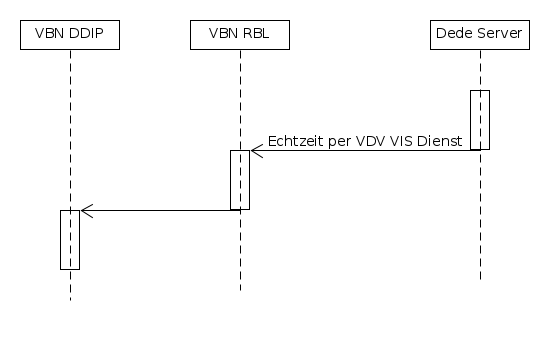
\includegraphics[width=0.75\paperwidth]{dede/dede-vbn-ddip}
\end{frame}
